\documentclass[runningheads]{llncs}

\usepackage{amssymb}
\setcounter{tocdepth}{3}
\usepackage{graphicx}

\usepackage{url}
\newcommand{\keywords}[1]{\par\addvspace\baselineskip
\noindent\keywordname\enspace\ignorespaces#1}

\usepackage{url}
\urldef{\mails}\path|{david.pastor,yves.raimond, mark.sandler}@elec.qmul.ac.uk|
%\newcommand{\keywords}[1]{\par\addvspace\baselineskip
%\noindent\keywordname\enspace\ignorespaces#1}

\begin{document}

\mainmatter

\title{A Logic-Based Framework for Digital Signal Processing}

\titlerunning{A Logic-Based Framework for Digital Signal Processing}

\author{David Pastor\and Yves Raimond\and Mark Sandler}

\institute{Centre for Digital Music, Queen Mary, University of London,\\
\mails}

\maketitle


\begin{abstract}
In this paper we describe a logic-based framework for Digital Signal Processing. This framework is implemented on SWI-Prolog and is formed of interfaces with different DSP libraries and APIs extending this logic language ``to speak'' DSP. This approach presents the advantage, in respect of other integrated APIs, of being application implementation independent, so the extended logic language can be loaded an embedded in any application or language interfacing SWI-Prolog. The new DSP capabilities are public as predicates grouped in modules which offer different levels of abstraction. Low-level modules offer predicates to communicate directly with the API. Task-oriented modules define some default routines which specific goals and procedures. Finally we can relate input/output through ``black boxes'' representing a semantic relationship between them. Modules can communicate by using commong semantic data types declared as functors which determine the possible workflows. Such a framework allow us to build complex DSP queries as procedures as well as simplify the extraction of audio processing knowledge with common semantics. Finally, Concurrent Transaction Logic allows us to wrap the procedural meaning of predicate rules into a declarative definition of transactions controlling the execution and updating of the processes.
\keywords{DSP predicates, computation query, computation reasoner, DSP scenarios, RDF}
\end{abstract}

\section{Introduction}\label{sec:intro}

Digital signal processing is a broad field and an object of an important research. Withing this research community, particular investigators are discovering and developing new algorithms for signal processing and analysis. Many projects aim at developing formal APIs providing a framework for algorithms implementation and publication. However, these APIs are normally designed as a closed environment which hardly interacts with other related APIs and applications. Although several APIs are wrapped and exported as ``plugin'' libraries which can be embedded in different applications, they still require the implementation of specific and non-interactive hosts.

This situation leads to many isolated applications, environments and sources of data working independently from each other. Any effort to combine them to obtain integrated results for analysis, classification and comparison requires tedious studies or ``glue code'' implementations.

In this paper we address this problematic situation by proposing and developing SWI-DSP, a logical framework for \textit{Audio Processing} (as subset of DSP) that extends the SWI-Prolog vocabulary. We rely on a logic programming language with aggregated audio analysis capabilities getting rid of the application-dependency paradigm and offering a single logic front-end which is generally more understandable than a closed implementation in any Procedural or Object Oriented language. In addition to this, we are keen on using logic resources to finally achieve a more capable DSP engine.

In \S 2 we identify the most common audio analysis tasks and summarize several relevant \textit{open source} APIs aimed at performing such tasks. We evaluate the advantages and limitations of these APIs in order to find the requirements for SWI-DSP. In \S 3 we start viewing the system from the top and how it defines an interesting workflow that characterizes input/output relationships between task-oriented modules. This workflow is determined by semantic types, a binary data standard and procedural declarations of DSP rules. \S 4 goes into the implementation of each task-oriented module which are indeed communication layers with dedicated ``plugin'' libraries that are in charge of the actual computation and offer an open development framework.

Thus, SWI-DSP extends SWI-Prolog vocabulary to perform audio analysis and processing by defining semantic types and predicates, triggering external computation performed by dedicated APIs, which are ordered in modules with different levels of abstraction. However, this front-end does not present an efficient and manageable framework as it requires specific SWI-Prolog knowledge to create programs suitable for the concrete needs and it does not offer any efficient tabling mechanism. We tackle this problem in \S 5 by defining DSP ``scenarios'' which offer a semantic view of the system to the user without losing computational flexibility. 

We also describe as a Standard, how Concurrent Transaction Logic is the solution to provide an efficient engine allowing a formal data updating mechanism and computation reasoning capabilities. Finally, \S 6 presents related works that use SWI-DSP to create an environment for multimedia data management and visualisation. We conclude in \S 7 by assessing the value and scope of this work and introducing future advances.

\section{Audio Analysis tasks and solutions}\label{sec:tasks}

Audio analysis and synthesis APIs offer formal implementations for development and use of different algorithms and techniques. These algorithms are focused on different tasks that can be classified in these 3 groups:

\begin{itemize}
 \item Processing and Effects
 \item Feature Extraction
 \item Classification
\end{itemize}

\subsection{Audio Processing}\label{subsec:effects}

This tasks group can be characterized by having audio signals as input and output, so an input signal is processed in such a way that we retrieve an altered, processed version of the original signal. Some examples of audio processing tasks are filtering, effects processing and signal generation.

One important dedicated API is the Linux Audio Developer's Simple Plugin API (LADSPA) which has been succesfully used in many systems and applications and is a widely spread implementation for algorithms development. We host LADSPA in SWI-DSP but there are other interesting libraries like DSSI plugins for effects and LV2 (new generation of LADSPA) which are targets for future extensions. (this is too simple i think)

\subsection{Feature Extraction}\label{subsec:feature}

Feature extraction is an important paradigm in signal research as it focuses on extract qualitative characteristics of the signal in a different domain than the input. Features are classified in different levels of abstraction from frequency and time domain characteristics to high-level audio ones.

The Vamp Plugins API offers a standard and utilities to develop feature extraction plugins that can be hosted in any application able to control the ``plugin lifecycle''. We host Vamp plugins as basis for feature extraction in SWI-DSP. In general plugin libraries are characterized for being easy for development but application-dependent. By embedding plugins in SWI-DSP we offer a flexible development framework and make an interactive interface to deal with plugins in several ways.

\subsection{Integrative solutions}\label{subsec:inte}

With the same motivation of this work there are some integrative APIs which combines different tasks to perform low high-level operations in a closed implementation. CLAM, jMIR and Marsyas present a complex framework collecting tools to perform different DSP tasks. The most interesting feature of these frameworks is the possibility to create DSP networks combining specific algorithms and modules thanks to a workflow design.

CLAM also offers a metamodel of DSP processes wich provides semantics to design the networks properly presenting a higher and more manageable level of abstraction. However, these APIs still present two important limitations that we pretend to solve:

\begin{itemize}
 \item There do not offer a common format to exchange data or an easy way to interact with other applications.
 \item They offer a procedural system unable to reach higher-level knowledge by itself.
\end{itemize}

\subsection{Classification}\label{subsec:classif}

Classification is one the most interesting and complex paradigms in any specific domain exploiting the ``intelligence'' of computational machines. The WEKA API collects different machine-learning algorithms and provides a formal interface (in Java) for development and interaction with other systems.

However, this generic API does not provide semantics to create a dataset which is the most intriguing and complex issue for classifying data properly. Marsyas and jMÍR integrate WEKA orienting it for music classification purporses by offering a code interface with other modules (Marsyas) or by extending the WEKA file format ARFF (jMIR). Both solutions still seem to lack of effective semantics to perform classification of audio data.

\section{SWI-DSP workflow}\label{sec:dspworkflow}

We find of high interest the workflow architecture for DSP tasks. A complex task is then subdivided into subgoals that are achieved for the specific task-oriented modules. A procedure of this nature can be easily implemented combining high-level predicates with a proper matching of the instantation patterns. These instantation patters must have terms in common which are easily carried forward from one module to another without worring about further conversion. For this purpose, we define semantic datatypes as SWI-Prolog functors. In the same sense, we need to define a standard format for large binary data objects which are highly common in DSP tasks. We define these utils in the \textbf{swilib} module which provides a C++ library and a SWI-Prolog module for their management.

\subsection{Semantic datatypes}\label{subsec:datatypes}

SWI-Prolog functors are defined by their name and their arity. Therefore we need to recognize and set the common concepts and their properties used in audio analysis. In the previous section we have seen how tasks are strongly characterized by the type of input and output. We also want to look at the Music Ontology specification [x] as ontological description of music-related concepts including audio analysis terminology. We distinguish the following semantic datatypes:

\begin{itemize}
 \item 'Signal'(Channels, SampleRate, Samples, [ListOfPCMPerChannel]): any audio data fragment is classified as a signal. Audio data is presented in our system as Pulse Code Modulation (PCM) which is a digital version of an analog signal sampled in equal intervals. Necessary parameters to understand the signal are the number of channels, the sample rate of the sampling and the resulting number of samples.

\item 'Frame'(Channels, SampleRate, StartingSample, [ListOfPCMPerChannel]) as pieces of a signal, frames have an important role in DSP as we need to decompose the signal in smaller frames for an efficient analysis.

\item 'Feature'(Type, Timestamp, Data): extracted characteristics of a signal in some other domain are called features which are the main target of audio analysis at a low level. A feature term is characterized by the feature type, its interval of time and the actual feature data.

\item 'Timestamp'(Start, Duration): audio properties are always necessarily bound to an interval of time defined as a timestamp in respect of the audio signal ``timeline''. 

\item 'Parameter'(Name, Value): parametrization of algorithms is one of the most significant issues in DSP as well. Algorithms vary their perfomance depending on the parameters. We want to generalize the parameterization for any task with generic terms.
\end{itemize}

\subsection{Large Binary Objects}\label{subsec:blobs}

The so called BLOBs are objects wrapping large binary data. The representation of data in SWI-Prolog can be done through lists which can not handle such amount of data (e.g. signals of 1000000 samples) or through BLOB terms which are cumbersome as datatype.

We have implemented a mechanism of \textit{data identifiers} that vary incrementally and are stored in a database updated in each session. These identifiers, with the form \textbf{data\_x}, hide the binary data (which is internally a vector of floats) and allow us to perform different operations over the data easily with prolog predicates: \textit{data\_out(+Id, +File), data\_in(+File, +Id), data\_to\_list(+Id, -List)...} as well as control the binary data database status. Each module is implemented to read/write data in this fashion.

\subsection{Workflow}\label{subsec:worflow}

These standards allow us to work with different modules without taking care of the specific underlying APIs types or implementation, so that we achieve a logic framework with dedicated semantics to perform audio analysis tasks as showed in \ref{fig:workflow}.

\begin{figure}
\centerline{\framebox{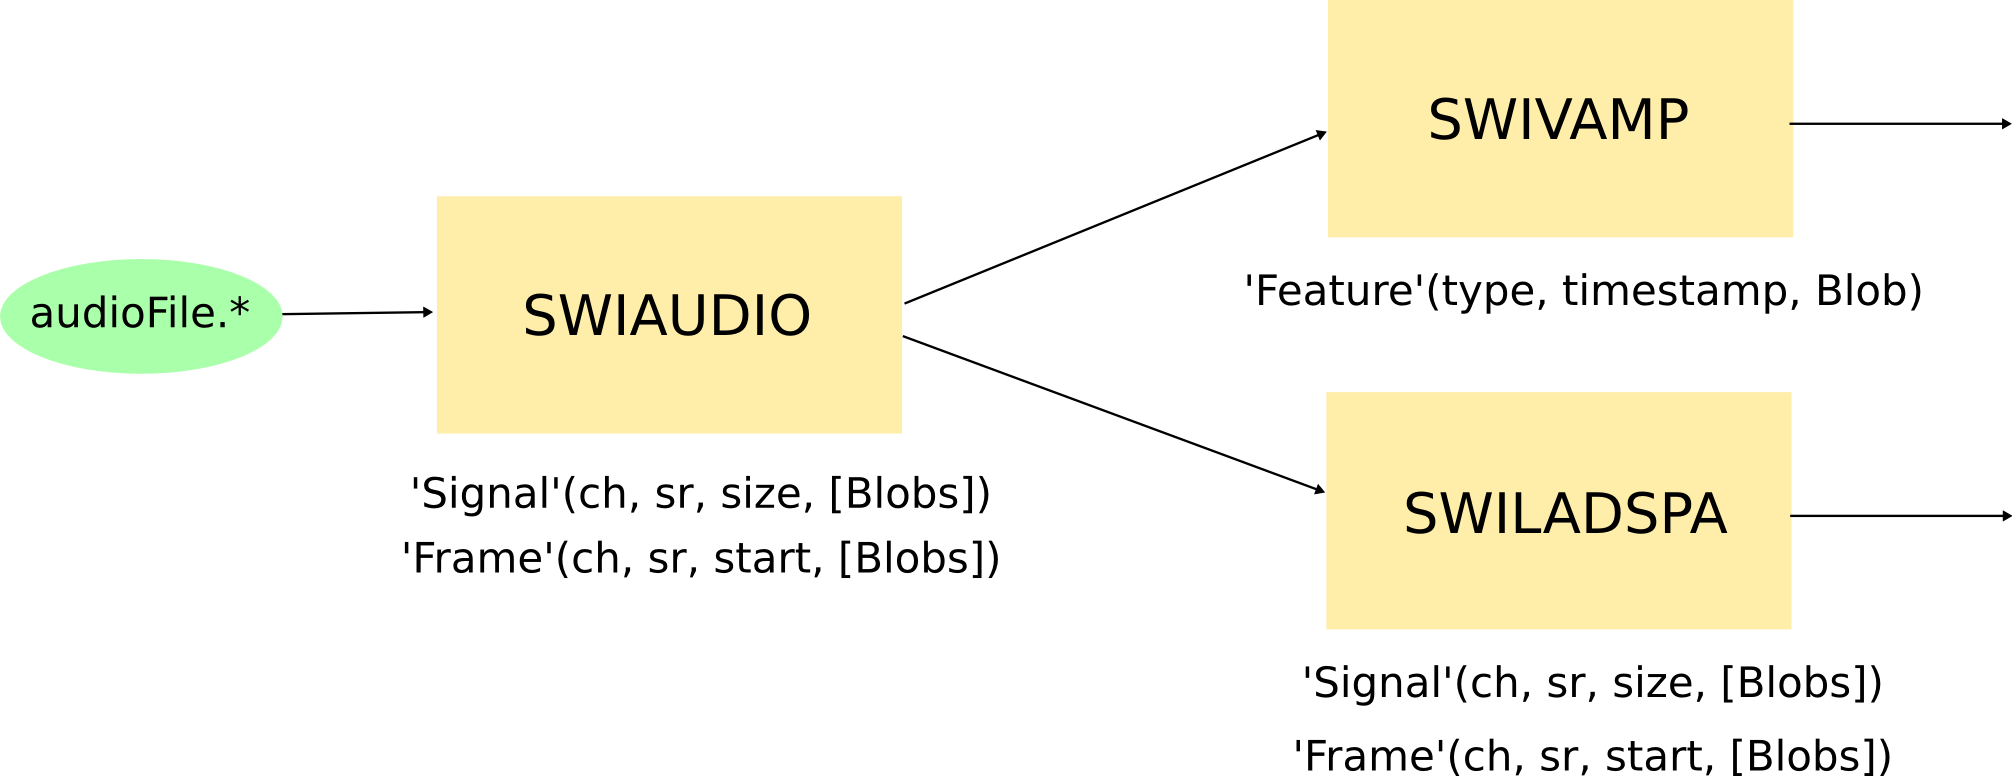
\includegraphics[width=\columnwidth]{workflow.png}}}
\caption{Workflow specification of the modules}
\label{fig:workflow}
\end{figure}

We can then execute the following task as a SWI-Prolog query. \textit{The input audio file is decoded and then we apply a pre-processing in which we amplify the signal. We then apply a key detection algorithm over the signal to retrieve tonal regions}

\begin{verbatim}
 
my_task(Input, ['Parameter'(gain, 2)], KeyProfile):-
	decode(InputFile, Signal),
	amplify(Signal, 'Parameter'(gain, 2), SignalX2),
	key(SignalX2, KeyProfile).

KeyProfile = ['Feature'(key, 'Timestamp'(0, 23.45), 'Amajor')|...].	

\end{verbatim}

\section{SWI-DSP modules}\label{sec:modules}

Each task module is composed by lower level modules which offer communication with an external API or library in charge of the computations. By hosting ``plugin libraries'' we can extend easily SWI-DSP vocabulary as we do not need to assemble each algorithm.

\subsection{swiaudio}\label{subsec:swiaudio}

This module is in charge of providing audio data to the system. This module is splitted in two sub-modules: \textbf{swiaudiosource} and \textbf{swiaudiodata}. The former is a powerful module for decoding which interacts with C decoding libraries (mad, soundfile, fishsound, oggz and faad) to extract a \textit{Signal} term given and audio input file supported by the libraries. This process is triggered by a simple call to the predicate \textit{aspl\_decode(+InputFile, -Signal)} which recognizes the file extension and calls a specific library allowing a fast decoding process and even more important an independent term representing the encoded data in a standard way for any format.

The latter is a module which defines utilities typically required in DSP. The most important set of predicates is dedicated to framing. The original signal is decomposed in overlapping blocks of data outputting frame terms through the non-deterministic predicate \textit{framing(+Signal, +StepSize, +BlockSize, -Frame)}. The rest of predicates are mainly oriented to extract information from a Signal or Frame term.
 
\subsection{feature extraction}\label{subsec:swivamp}

This module defines a standard task-oriented set of predicates for feature extraction. As we have seen in \S 2 the module is characterized for a clear input/output relationship. So we can declare a simple predicate to extract the tempo of an audio signal: tempo(+Input, -Tempo) being Input an instantation of the Signal datatype and Tempo a list of instantations of the Feature datatype. This ``magic'' predicate is triggering a specific computation tool, so we could select the specific tool by extending the predicate: \textit{tempo(+Input, +Tool, -Tempo)}.

We rely on the Vamp Plugin API as it offers an efficient plugin and host implementation. Certainly, there is a limitation in the sense that any feature extraction algorithm we may want to use has to be implemented as Vamp Plugin, but as counterpart it is easier to write an algorithm as Vamp Plugin than to interface many APIs or particular algorithm implementations.

The sub-module \textbf{swivamp} is a communication layer based on the SWI-Prolog foreign interface which allow us to query the plugin information, set up the plugin context for the transform, execute the plugin given a Signal term and retrieve the output features for the plugin according to the lifecycle specification. Plugins are wrapped in a similar fashion than the audio data so we can use a plugin instance representation which allow us to have concurrent plugins working at the same time. The previous tempo/3 predicate is declared as this set of rules:

\begin{verbatim}

tempo(Input, Tool, Tempo):-
        Input = 'Signal'(Ch, Sr, L, PCMs),
        Tool = 'Vamp',
        vamp_feature_of('tempo', Signal, WholeFeature).
vamp_feature_of(Type, Signal, WholeFeature):-
        select_plugin(Type, PluginKey, Output),
        vamp_outputs_for(Signal, PluginKey, Output, Features),
        flatten(Features, WholeFeature).
vamp_outputs_for(Signak, PluginKey, Output, Feature):-
        vmpl_load_plugin_for(PluginKey, Signal, Plugin),
        set_blockSize(Plugin, BlockSize),
        set_stepSize(Plugin, StepSize),
        get_channels(Signal, Channels),
        vmpl_initialize_plugin(Plugin, Channels, StepSize, BlockSize),
        vamp_compute_feature(Signal, StepSize, BlockSize, Outputs, Plugin, WholeFeature).
vamp_compute_feature(Signal, StepSize, BlockSize, Outputs, Plugin, WholeFeature):-
        get_samples_per_channel(Signal, L),
        findall(Features, vamp_process_signal(Signal, L, StepSize, BlockSize, Output, Plugin, Features), FeatureSet),
        get_sample_rate(Signal, SampleRate),
        vmpl_remaining_features(Plugin, L, SampleRate, Output, Remaining),
        append(FeatureSet, Remaining, RawFeatures),
        delete(RawFeatures, [], WholeFeature).
vamp_process_signal(Signal, L, StepSize, BlockSize, Output, Plugin, Features):-
        set_limit_framing(L, StepSize, Limit),
        set_framing(StepSize, L, Limit, Start),
        vmpl_process_block_framing(Plugin, Signal, Start, BlockSize, Output, FeatureSet).

\end{verbatim}

\subsection{audio processing}\label{subsec:swilasdpa}

This module defines any computation which outputs a Signal term. This 

The module swiladspa offers communication with LADSPA which is the most generic and spread plugin API for general audio processing.

\subsection{swiweka}\label{subsec:swiweka}

\section{Towards a computation reasoner}\label{sec:reasoner}

So far we have presented how SWI-DSP provides a vocabulary of logic predicates to perform audio analysis computations, but this logic front-end is still inappropiate for such tasks. We have organized the modules in communication layers and task-oriented modules, but there is an important trade-off between understandability and specification. The communication layer even offering an application-independent access to the computation libraries still requires a high knowledge of such libraries besides a SWI-Prolog familiarization which is not expected in most part of the potential users. The task-oriented module which is itself very layered provides high-level predicates which are missing some important options at setting-up. 

In addition to this, we need require a mechanism to update results and keep track of computation sequences, so that computations are not restricted to one SWI-Prolog session, allowing us to reuse and share them. This section tackles this problem by extending SWI-DSP as an expert system with defined ``DSP scenarios'' and by introducing Concurrent Transaction Logic on top of our extended predicate-logic language.

\subsection{DSP scenarios}\label{subsec:scenarios}

Our DSP workflow is strongly constrained by the predicate instantation patterns which clearly establishes a hierarchy of users depeding on the level of abstraction we are dealing with. Applications provide the user with a nice graphical or command line interface to control the computations. We need therefore to set a ``nice view'' of the system to the potential users which are not (and do not need to be) related to the SWI-DSP or the libraries implementation.

We address this problem by defining ``scenarios'' that control and delimit the user's view of the system without restricting significantly his options. Any computation over an audio signal can be seen as a function input/ouput with a specific setup. The ``scenario'' characterizes such a family of funtions in a generic way so the user just needs to configure the scenario and provide the input to capture the output. Such computations can be wrapped as a signal \textbf{transform} which is declared as a SWI-Prolog functor:

'Transform'(TransformType, 'Engine'(API, PluginName, Version), SampleRate, StepSize, BlockSize, ListOfParameters, Program).

\begin{itemize}

 \item TransformType indicates which sort of task we are carrying out (feature extraction, audio effect...)
 \item 'Engine'(A, Pn, V) identifies the computation engine in charge of the processing of the transform
 \item SampleRate indicates the input sample rate in case it is not constant
 \item StepSize and BlockSize are the framing parameters
 \item ListOfParameters to setup the engine
 \item Program is a predetermined configuration for the engine
\end{itemize}

Then each task module hardcodes the necessary knowledge in form of interpretation rules to read the tranform scenario and set the up the corresponding engine. The predicate \textit{transform(+InputSignal, +TransformContext, -Output)} will provide a generic view of processing to the user with standarized semantics.

Another complex ``scenario'' is classification. We find this approach suitable to control swiweka effectively. Each classification context can be defined by:

'Classification'(Identifier, ListOfCategories, ListOfDataRecords, Classifier, Classification) (have to look at it better)

\subsection{Computation reasoning}\label{subsec:ctl}

The previous abstraction of computations offers a cleaner view of the system without loosing flexibility but there are more issues to be addressed. The system proposed so far does not provide anything novel in respect of other approaches presented in \S 2 and even could seem even more cumbersome to deal with. The major advantage of using a logic framework as basis of the DSP system is the reasoning capability of such a framework. 

This reasoning skills are extended to computation reasoning by using the Concurrent Transaction Logic as superset of the Predicates Logic. Transaction Logic defines the logics that allow us to control and manage the execution of the computation and reason about the effects in these terms:

\begin{itemize}
 \item Integration of updating transactions in queries with formal logics
 \item Integration of declarative and procedural meanings of computational transactions (paths)
\end{itemize}

The extended syntax provides connectives for different program states to create a complex execution path (allowing parallel/serial operations, concurrency control, loops, conditionals, recursion and subroutines). The declarative meaning and the procedural meaning are combined:

computation A executes along path X = A is true on X

Actually we are now in position to define several execution paths for the same computation, control the execution of those paths, reason about the results and the truth of such executions and store the computation sequences and data states.

(need one good example here)

\section{SWI-DSP in real applications}\label{sec:realapp}

SWI-DSP defines therefore a logic front-end for computations in DSP ``scenarios''. We have described how Concurrent Transaction Logic converts this framework based on a predicate calculus into a DSP reasoner which control the execution and data of the different scenarios. This system still needs an implementation which allow an external user to control easily the reasoner, access the computations and visualise the results.

\subsection{Languages hosting SWI-Prolog}

.... comment possible languages interfacing prolog...

\subsection{Henry}\label{subsec:henry}

Although SWI-Prolog is a well-known and used implementation of Prolog it does not represent the most suitable framework to deal with multimedia data. The multimedia community in general needs a standard machine-readable format with proper semantics to manage data. The Resource Description Framework (RDF) has been proposed as such a format and defines an Standard to represent linked data by means of triples in the form of (Subject, Predicate, Object).

This standard can be implemented with different syntaxes. We prefer to use Notation3 [x] whose syntax allow us to write RDF statements in a human-readable way and also to write ``rules'' as named graphs [g]. This is a suitable framework to represent data that can be shared and published in the so-called ``web of data``.

The Ontology Web Language (OWL) provides the framework to express the knowledge of a particular domain in RDF through concepts and relationships. Thus, descripting semantic models related to audio analysis are not restricted to a local implementation but can be shared and processed by different systems.

The project called Henry implements an N3/Prolog parser and reasoner based on Concurrent Transaction Logic. This agent defines an entailment module capable of reasoning over the SWI-DSP computations, which are identified through Universal Resource Identifiers (URIs), and N3 statements and rules. The semantic web package module for SWI-Prolog interprets SPARQL queries which are passed to Henry which produces RDF descriptions of computations by performing the entailment and triggering SWI-DSP computations. 

(any example or figure maybe)

 \section{Conclusion and Future work}\label{sec:conclusion}

We have presented a powerful reasoner for multimedia analysis implemented as a logic-based framework that aims at converting low-level computations into shareable and distributed knowledge.

\end{document}
